\documentclass{article}
\usepackage{graphicx} % Required for inserting images
\usepackage[polish]{babel}
\usepackage[T1]{fontenc}
\usepackage{amsmath}
\usepackage[utf8]{inputenc}
\usepackage{minted}
\graphicspath{{./images/}}
\usepackage{listings}
\usepackage{amssymb

\title{Teoria Współbierzności - Zadanie domowe 3}
\author{Jakub Frączek}
\begin{document}

\maketitle

\section{Opis zadania}

Zadanie polegało na kolejno:

\begin{enumerate}
    \item Zlokalizowaniu niepodzielnych czynności wykonywanych przez algorytm eliminacji Gaussa, nazwać je oraz zbudować alfabet w sensie teorii śladów
    \item Skonstruowaniu relacji zależności dla alfabetu, opisującego algorytm eliminacji Gaussa. 
    \item Przedstawieniu algorytmu eliminacji Gaussa w postaci ciągu symboli alfabetu.
    \item Wygenerowaniu grafu zależności Diekerta
    \item Przekształceniu ciąg symboli opisującegi algorytm do postaci normalnej Foaty.
    \item Zaprojektowaniu i zaimplementowaniu współbieżnego algorytmu eliminacji Gaussa.
\end{enumerate}

\section{Wykorzystane technologie}
Do implementacji zadania został wykorzystany język Python w wersji 12.3.8 oraz moduły:

\begin{itemize}
    \item sys
    \item os
    \item warnings
    \item time
    \item itertools
    \item python-graphviz 0.20.1
    \item numpy 1.26.4
    \item numba 0.60.0
\end{itemize}

\section{Dane techniczne}

Testy algorytmu zostały przeprowadzone na komputerze z 64 bitowym systemem Windows 11, procesorem Intel Core i5-9300H 2.40 GHz, kartą graficzną Geforce GTX 1650 oraz 32 GB pamięci RAM.

\section{Realizacja zadania}

\subsection{Część teoretyczna}

W algorytmie eliminacji Gaussa można wyróżnić trzy niepodzielne operacje:

\begin{itemize}
    \item \(A_{a, b}\) - wyznaczenie ilorazu elementów macierzy: \(M[b][a] / M[a][a]\)
    \item \(B_{a, i, b}\) - wyznaczenie iloczynu: \(M[a][i]  * A_{a, b}\)
    \item \(C_{a, i, b}\) - wyznaczenie różnicy i przypisanie do elementu: \(M[b][i] = M[b][i] - B_{a, i, b} \)
\end{itemize}

\subsection{Część implementacyjna dotycząca teorii śladów}

Pierwszym etapem było napisanie funkcji \text{calculate\_operations}, która wyznacza listę kolejnych operacji na rzędach macierzy jakie powinien wykonać algorytm Gaussa w celu otrzemania macierzy trójkątnej górnej. Wyznaczona lista po spłaszczeniu za pomocą funkcji \text{get\_alphabet} zawiera unikalne symbole, które jednoznacznie wyznaczają alfabet w sensie teorii śladów oraz słowo w opisujące kroki algorytmu. Następnie wykorzystując funkcję \text{get\_dependence} wyznaczam relację zależności, uwzględniając przy tym jedynie bezpośrednie zależności między operacjami. Kolejno na podstawie wyznaczej relacji i alfabetu wyznaczam graf Diekerta za pomocą funkcji \text{diekert\_graph}, a następnie klasy foaty dzięki funkcji \text{get\_foaty}. Na końcu dzięki bibliotece \text{python-graphviz} rysuję wyznaczony graf Diekerta.

\subsection{Część implementacyjna dotycząca algorytmu Gaussa}

Do implementacji współbieżnej części algorytmu skorzystałem z modułu \text{numba} pozwalającego na napisanie funkcji wykonywanych na rdzeniach CUDA. Są to:
\begin{itemize}
    \item \text{gaussian\_elimination\_A\_kernel} - wykonująca operację \(A_{a, b}\)
    \item \text{gaussian\_elimination\_B\_kernel} - wykonująca operację \(B_{a, i, b}\)
    \item \text{gaussian\_elimination\_C\_kernel} - wykonująca operację \(C_{a, i, b}\)
\end{itemize}

\noindent
W pętli w funkcji \text{gaussian\_elimination\_cuda} kolejno wykonuję współbieżnie wszystkie operacje znajdujące się w jednej klasie Foaty wykorzystując wyżej wymienione funkcje. Finalnie wyliczam rozwiązanie układu już na CPU za pomocą funkcji \text{to\_identity\_and\_solve}.


\section{Wyniki}

\subsection{Dla przykładowego wejścia}

W treści zadania podane zostało przykładowe wejście do programu:

\begin{minted}[bgcolor=white, frame=single, fontsize=\small]{python}
3
2.0 1.0 3.0
4.0 3.0 8.0
6.0 5.0 16.0
6.0 15.0 27.0
\end{minted}

\noindent
Otrzymane wyniki:


\begin{flalign*}
\Sigma = \{ & A_{1 2}, B_{1 1 2}, C_{1 1 2}, B_{1 2 2}, C_{1 2 2}, 
B_{1 3 2}, C_{1 3 2}, B_{1 4 2}, C_{1 4 2}, A_{1 3}, \\
& B_{1 1 3}, C_{1 1 3}, B_{1 2 3}, C_{1 2 3}, B_{1 3 3}, 
C_{1 3 3}, B_{1 4 3}, C_{1 4 3}, A_{2 3}, B_{2 2 3}, \\
& C_{2 2 3}, B_{2 3 3}, C_{2 3 3}, B_{2 4 3}, C_{2 4 3} \}
\end{flalign*}

\begin{flalign*}
D = sym\{
  &(A_{1 2}, B_{1 1 2}), (B_{1 1 2}, C_{1 1 2}), 
  (A_{1 2}, B_{1 2 2}), (B_{1 2 2}, C_{1 2 2}), \\
  &(A_{1 2}, B_{1 3 2}), (B_{1 3 2}, C_{1 3 2}), 
  (A_{1 2}, B_{1 4 2}), (B_{1 4 2}, C_{1 4 2}), \\
  &(A_{1 3}, B_{1 1 3}), (B_{1 1 3}, C_{1 1 3}), 
  (A_{1 3}, B_{1 2 3}), (B_{1 2 3}, C_{1 2 3}), \\
  &(A_{1 3}, B_{1 3 3}), (B_{1 3 3}, C_{1 3 3}), 
  (A_{1 3}, B_{1 4 3}), (B_{1 4 3}, C_{1 4 3}), \\
  &(C_{1 2 3}, A_{2 3}), (C_{1 2 2}, A_{2 3}), 
  (A_{2 3}, B_{2 2 3}), (B_{2 2 3}, C_{2 2 3}), \\
  &(C_{1 3 2}, B_{2 3 3}), (A_{2 3}, B_{2 3 3}), 
  (C_{1 3 3}, C_{2 3 3}), (B_{2 3 3}, C_{2 3 3}), \\
  &(C_{1 4 2}, B_{2 4 3}), (A_{2 3}, B_{2 4 3}),
  (C_{1 4 3}, C_{2 4 3}), (B_{2 4 3}, C_{2 4 3}) 
\}^+ \cup I_{\Sigma}
\end{flalign*}

\begin{flalign*}
t =[w]_{=_I^+} = &[< A_{1 2}, B_{1 1 2}, C_{1 1 2}, B_{1 2 2}, C_{1 2 2}, 
      B_{1 3 2}, C_{1 3 2}, B_{1 4 2}, C_{1 4 2}, A_{1 3}, \\
      &B_{1 1 3}, C_{1 1 3}, B_{1 2 3}, C_{1 2 3}, B_{1 3 3}, 
      C_{1 3 3}, B_{1 4 3}, C_{1 4 3}, A_{2 3}, B_{2 2 3}, \\
      &C_{2 2 3}, B_{2 3 3}, C_{2 3 3}, B_{2 4 3}, C_{2 4 3} >]
\end{flalign*}

\begin{flalign*}
 t =[⟨A⟩]_{=_I^+} = \{
  &[\{ A_{1 2}, A_{1 3} \}]_{=_I^+}  \\
  & \frown[\{ B_{1 1 2}, B_{1 2 2}, B_{1 3 2}, B_{1 4 2}, B_{1 1 3}, B_{1 2 3}, B_{1 3 3}, B_{1 4 3} \}]_{=_I^+} \\
  & \frown[\{ C_{1 1 2}, C_{1 2 2}, C_{1 3 2}, C_{1 4 2}, C_{1 1 3}, C_{1 2 3}, C_{1 3 3}, C_{1 4 3} \}]_{=_I^+} \\
  &\frown[\{ A_{2 3} \}]_{=_I^+} \\
  &\frown[\{ B_{2 2 3}, B_{2 3 3}, B_{2 4 3} \}]_{=_I^+} \\
  &\frown[\{ C_{2 2 3}, C_{2 3 3}, C_{2 4 3} \}]_{=_I^+}
\}
\end{flalign*}

\begin{figure}[H]
  \centering
    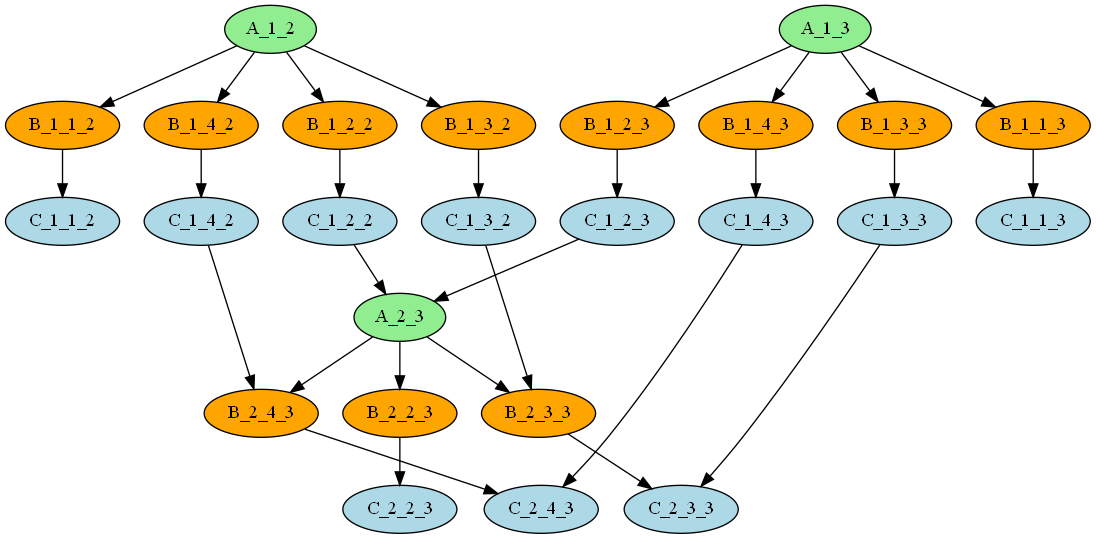
\includegraphics[width=0.99\textwidth]{images/diekert_graph_ex_3.png}
  \caption{Graf Diekerta dla danego przykładu}
\end{figure}

\noindent
Rozwiązanie układu równań:
\begin{minted}[bgcolor=white, frame=single, fontsize=\small]{python}
3
1.0 0.0 0.0 
0.0 1.0 0.0 
0.0 0.0 1.0 
1.0 1.0 1.0 
\end{minted}

\newpage

\subsection{Porównanie Grafu Diekerta dla różnych rozmiarów układu}

Na trzech poniższych wykresach znajduje się porównanie grafów Diekerta dla macierzy
o rozmiarach kolejno 4, 5, 6. Grafy dla każdej macierzy o tych rozmiarach będą wyglądać
tak samo bez względu na wartości.

\begin{figure}[H]
  \centering
    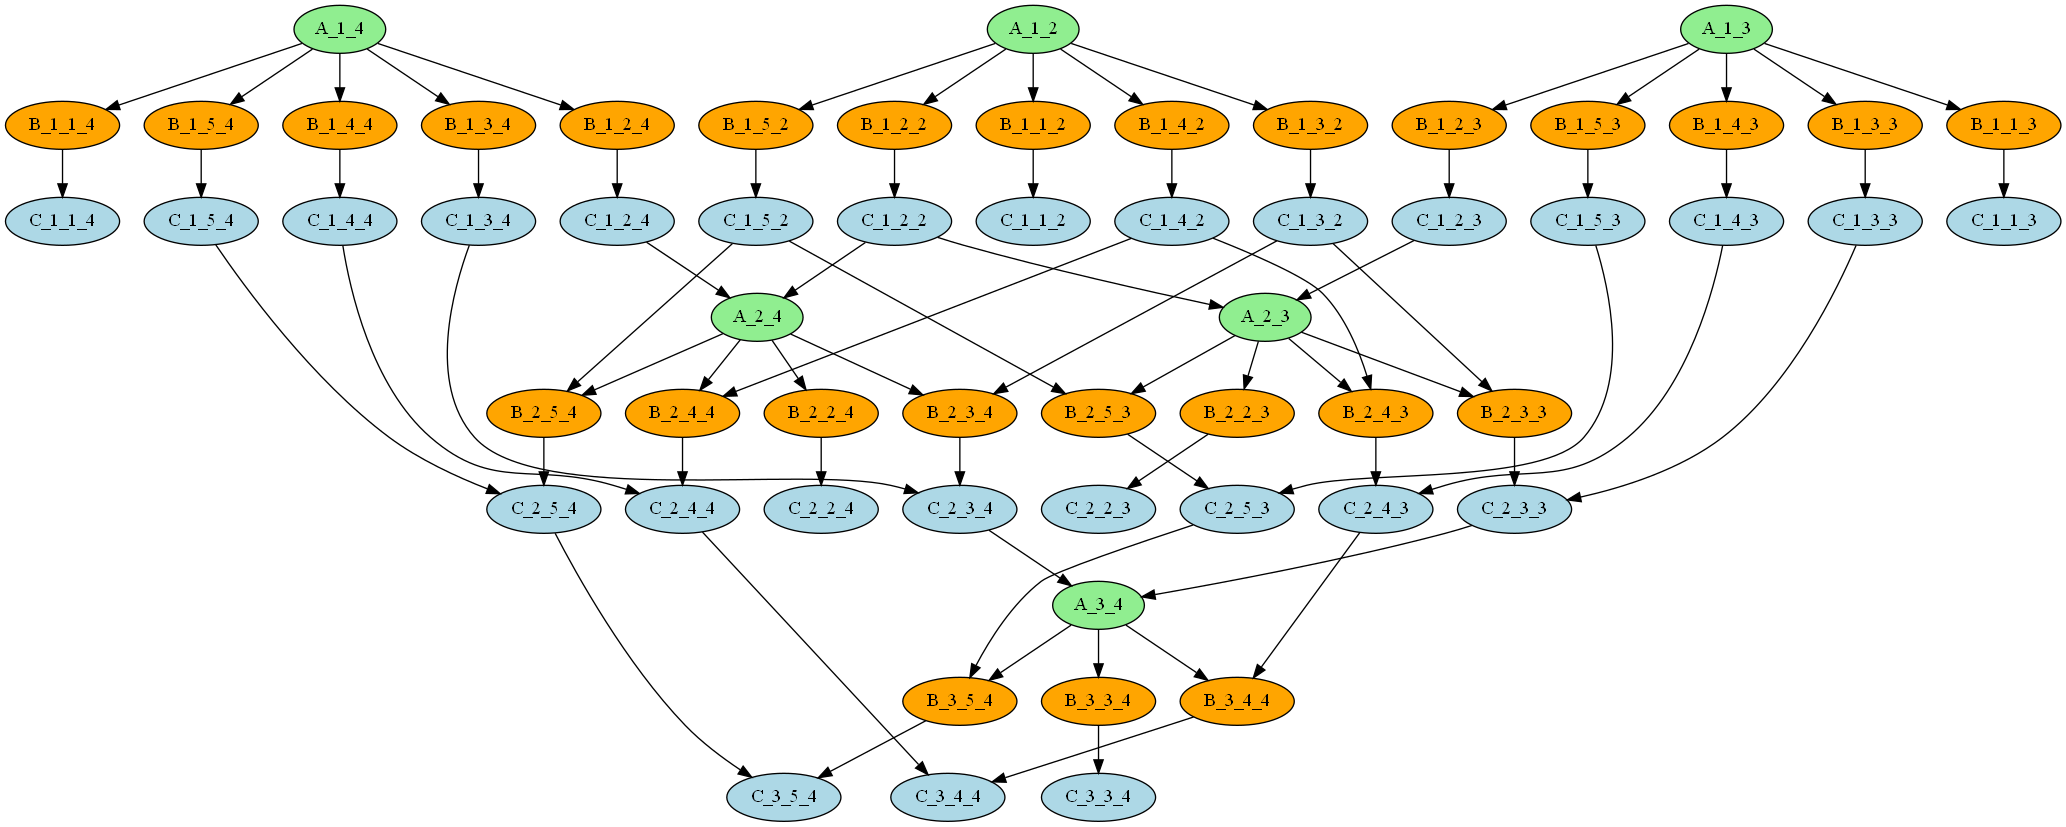
\includegraphics[width=0.99\textwidth]{images/diekert_graph_ex_4.png}
  \caption{Graf Diekerta dla macierzy o rozmiarze 4}
\end{figure}

\begin{figure}[H]
  \centering
    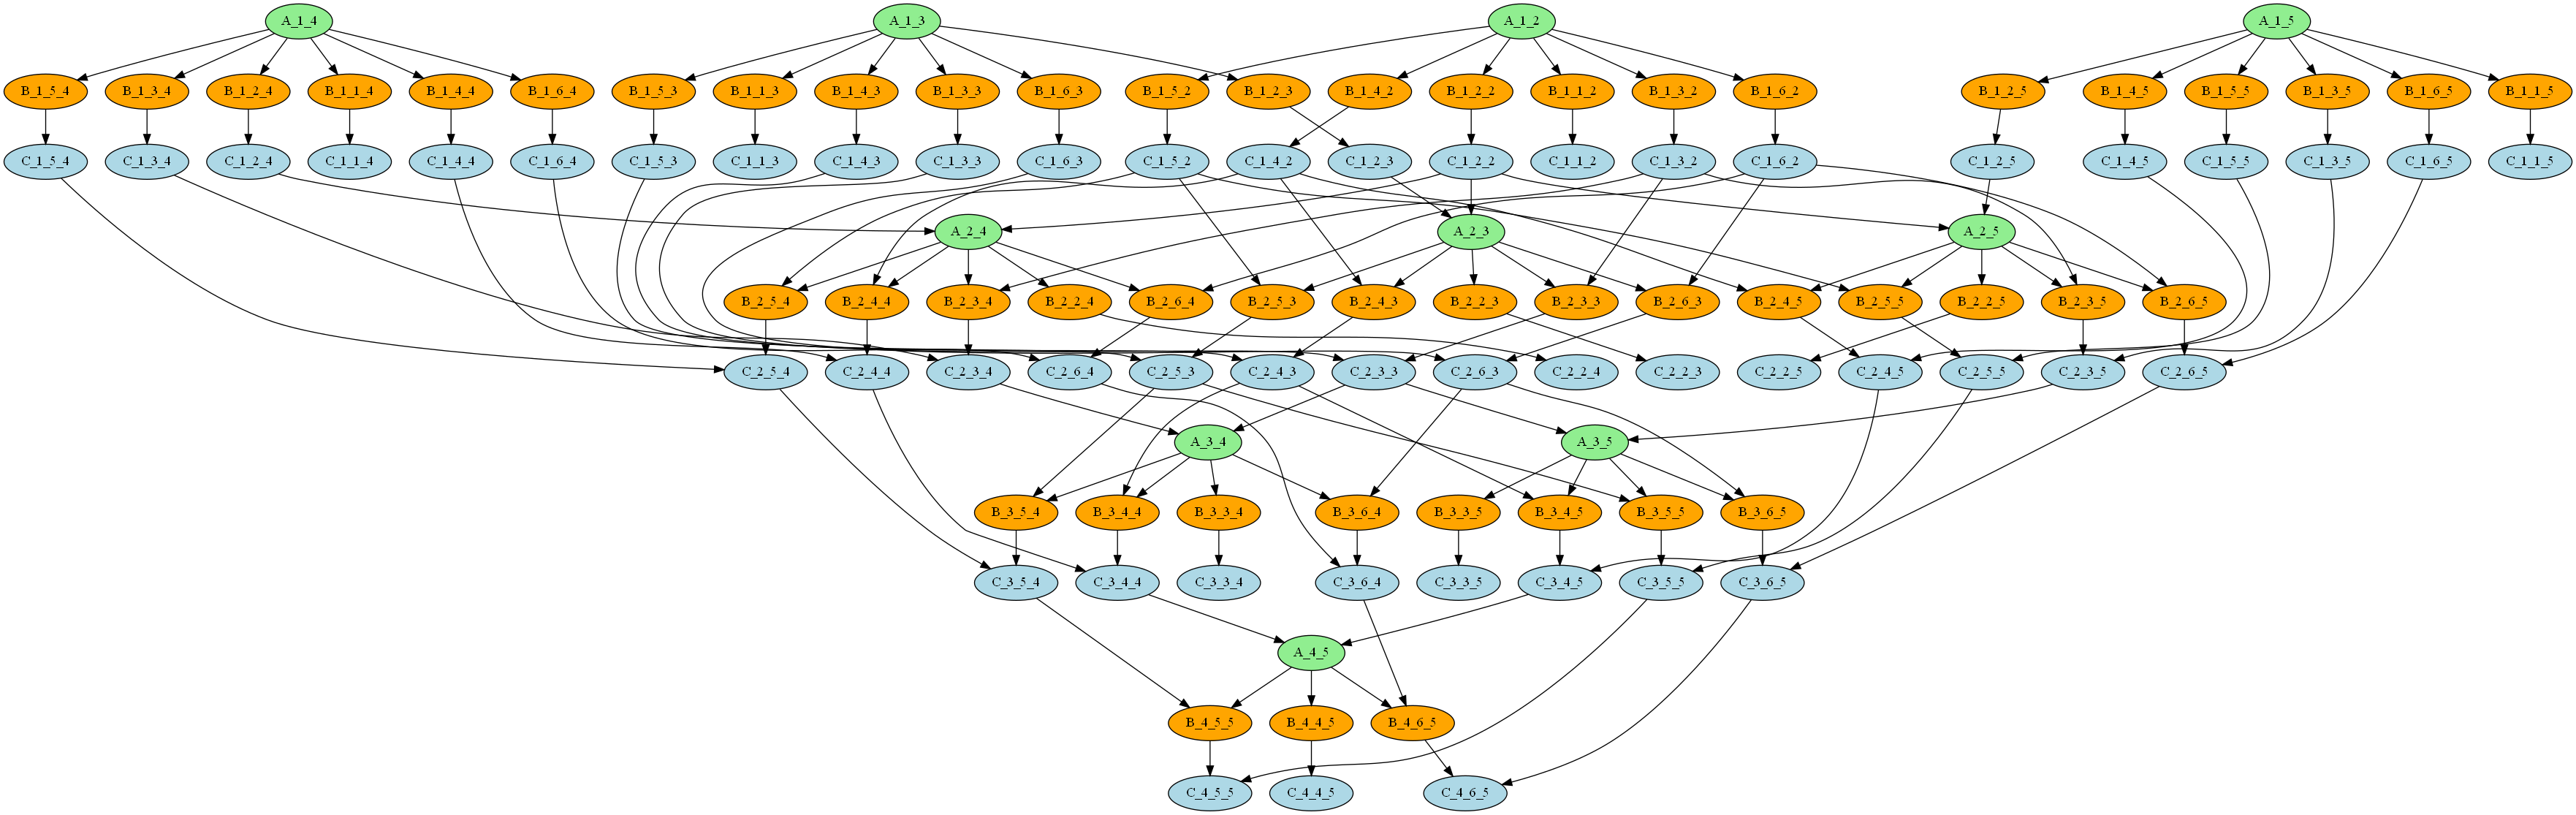
\includegraphics[width=0.99\textwidth]{images/diekert_graph_ex_5.png}
  \caption{Graf Diekerta dla macierzy o rozmiarze 5}
\end{figure}

\begin{figure}[H]
  \centering
    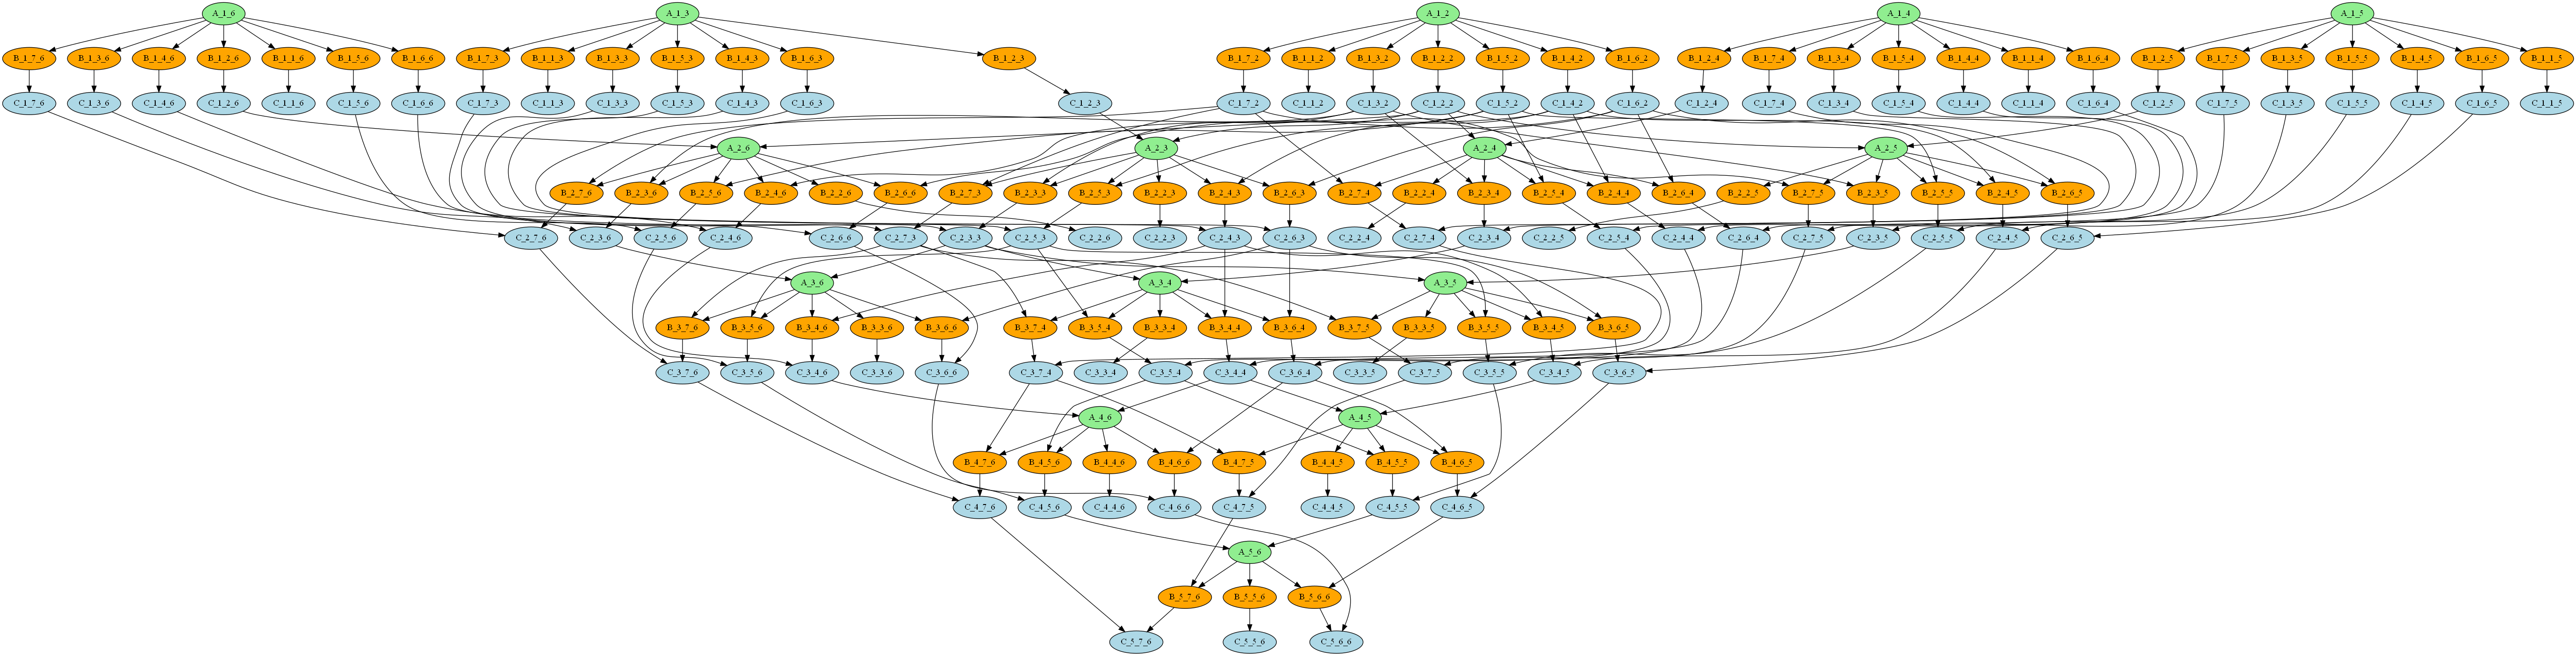
\includegraphics[width=0.99\textwidth]{images/diekert_graph_ex_6.png}
  \caption{Graf Diekerta dla macierzy o rozmiarze 6}
\end{figure}

\subsubsection{Testy ze sprawdzarką}

Przeprowadziłem testy dla różnych rozmiarów macierzy i za każdym razem otrzymany wynik był poprawny. Dodatkowo wykorzystując generator ze sprawdzarki przeprowadziłem testy czasów wykonania zaimplementowanego algorytmu Gaussa, co zostało pokazane na poniższym wykresie.

\begin{figure}[H]
  \centering
    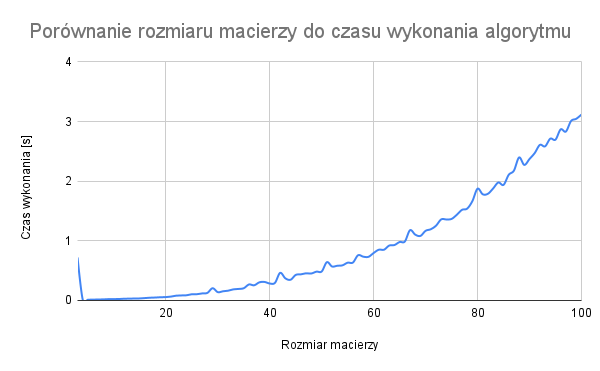
\includegraphics[width=0.85\textwidth]{images/time.png}
  \caption{Porównanie czasów działania algorytmu Gaussa do rozmiarów macierzy}
\end{figure}


\section{Wnioski}

\begin{enumerate}
    \item Zrozumienie i wykorzystanie teorii śladów pozwala na efektywne rozbicie problemu na części pierwsze, a następnie ich wykorzystanie do implementacji algorytmu współbieżnego
    \item Zadanie pozwoliło mi nauczyć się i zrozumieć jak działa uruchamianie kodu na GPU.
    \item Program poprawnie wyznacza obiekty matematyczne związane z teorią śladów oraz rozwiązuje układ równań.
\end{enumerate}

\section{Źródła}
\begin{itemize}
    \item Wykład z przedmiotu Teoria Współbieżności
    \item Materiały zamieszczone w sytemie UPEL
    \item https://developer.nvidia.com
\end{itemize}

\end{document}